\chapter{Structural Results}\label{chap:structural-results}


This chapter shall be devoted to looking at some structural results on arithmetic circuits. This would help us understand the relevance of shallow circuits in the context of proving lower bounds for arithmetic circuits of arbitrary depth. 

\section{Homogenization}\label{sec:homogenization}

Suppose we have an $n$-variate degree $d$ polynomial computed by an arithmetic circuit $C$. How large can the degree of intermediate computations be? Potentially, intermediate computations can involve very high degree terms which somehow cancel each other at the root. However, the following lemma of Strassen shows that we may assume without much loss of generality that arithmetic circuits never compute polynomials of degree more than the output. 

\begin{definition}[Homogeneous circuits]
A circuit $C$ is said to be \emph{homogeneous} if every gate in the circuit computes a homogeneous polynomial. 
\end{definition}

\begin{lemma}[Homogenization]
Let $f$ be an $n$-variate degree $d$ polynomial computed by a circuit $C$ of size $s$. Then, for every $0\leq i \leq d$, there is a \emph{homogeneous arithmetic circuit} $C_i'$, of size at most $O(sd^2)$, that computes the degree $i$ homogeneous polynomial in $i$. 
\end{lemma}
\begin{proof}
Assume without loss of generality that the circuit $C$ has all gates with fan-in at most $2$. 
For every gate $g\in C$, define $(d+1)$ gates $g^{(0)},\dots, g^{(d)}$; we shall construct a new circuit $C'$ such that $g^{(i)}$ computes the degree $i$ homogeneous part of the polynomial computed at $g$. If $g$ has children $h_1$ and $h_2$, then $C'$ would have the following connections depending on the type of the gate $g$:
\begin{eqnarray*}
\text{$g = h_1 + h_2$}\quad\implies\quad g^{(i)} &=& h_1^{(i)} \spaced{+} h_2^{(i)}\quad\text{for all $i$}\\
\text{$g = h_1 \times h_2$}\quad\implies\quad g^{(i)} &=& \sum_{j=0}^i h_1^{(j)} h_2^{(i-j)}\quad\text{for all $i$}
\end{eqnarray*}
It is easy to check that the size of the circuit $C'$ is at most $O(sd^2)$, and computes all the homogeneous components of $f$. 
\end{proof}

Thus, for arithmetic circuits, we can assume without much loss of generality that we are working with a homogeneous circuit. 

\begin{remark*}
For the class of arithmetic formulas, it is not clear if we can homogeneous without loss of generality. If we were to apply the above lemma to an arbitrary arithmetic formula, the resulting object is a homogeneous circuit and not a formula. It is unclear if any formula can be homogenized without loss of generality. The same is the case even for constant depth circuits, as the above construction does not preserve the depth of the circuit. 

However, the class of ABPs can also be assumed to be homogeneous without loss of generality. We leave this as an exercise. 
\end{remark*}

\begin{exercise}
Prove a similar homogenization lemma for arithmetic branching programs. 
\end{exercise}

\section{Depth reduction}

The phenomenon of simulating an arbitrary arithmetic circuit by a \emph{shallow} arithmetic circuit is called \emph{depth reduction}. Arithmetic circuits exhibit some remarkable depth reduction results, and we shall go over these in this section. 

\subsection{Depth reduction for arithmetic formulas}

The depth reduction for formulas is quite easy to describe. This would also serve as step towards understanding the depth reduction for arithmetic circuits. The following depth reduction is due to Brent~\cite{brent74}. 

\begin{lemma}[\cite{brent74}]
Let $f$ be an $n$-variate degree $d$ polynomial computed by an arithmetic formula $\Phi$ of size $s$. Then, $f$ can also be computed by a formula $\Phi'$ of size $s' = \poly(s,n,d)$ and depth $O(\log s)$. 
\end{lemma}
\begin{proof}
Assume without loss of generality that $\Phi$ is a formula of fan-in $2$. Starting from the root, walk down to the leaves by always taking the child with a larger sub-tree under it. Consider the first node in this path $v$ such that the size of the formula rooted at $v$ is smaller than $\frac{2s}{3}$. Let $\Phi_v$ refer to the sub-formula rooted at $v$. By the choice of the path from the root, we have
\[
\frac{s}{3} \spaced{\leq} \abs{\Phi_v} \spaced{<} \frac{2s}{3}.
\]
Let $\hat{\Phi}_v$ denote the formula where the sub-formula at $v$ is replaced by a fresh variable $y$. Since we are dealing with formulas, $\hat{\Phi}_v$ is a linear polynomial in the variable $y$. Hence,
\begin{eqnarray*}
\hat{\Phi}_v(y) & = & A \cdot y \spaced{+} B\\
\text{and,}\quad \Phi & = & A \cdot \Phi_v \spaced{+} B
\end{eqnarray*}
for some polynomials $A$ and $B$. But we can compute both $A$ and $B$ from $\hat{\Phi}_v(y)$ as
\begin{eqnarray*}
A & = & \hat{\Phi}_v(1) - \hat{\Phi}_v(0)\\
B & = & \hat{\Phi}_v(0)
\end{eqnarray*}
Thus, 
\[
f \quad = \quad (\hat{\Phi}_v(1) - \hat{\Phi}_v(0))\cdot \Phi_v \spaced{+} \hat{\Phi}_v(0)
\]
All the formulas in the above equation have size at most $\frac{2s}{3}$. Thus, by recursively applying this process on each of these sub-formulas, we obtain an $O(\log s)$ depth formula of size $\poly(s)$ as claimed. 
\end{proof}

\begin{figure}
\begin{center}
\tikzstyle{gate}=[circle,draw=black!50,thick]
\tikzstyle{leaf}=[circle,draw=black!50,fill=black!10,thick]
\tikzstyle{phi}=[rectangle,draw=black!50,fill=black!10,thick]
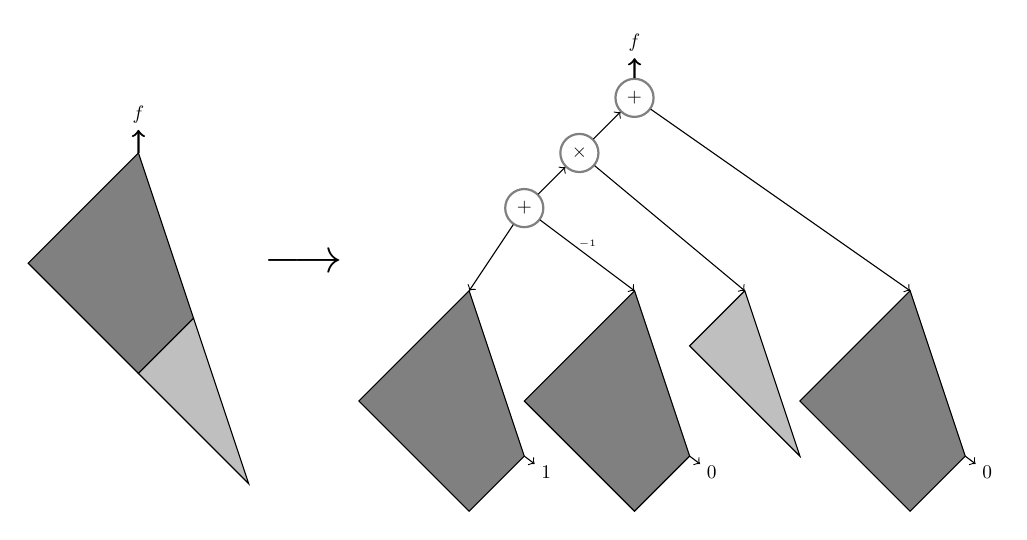
\begin{tikzpicture}[transform shape, scale=0.7]
  \draw[fill=gray] (-10,-2) -- ++(-2,-2) -- ++(2,-2) -- ++(1,1) -- cycle;
  \draw[fill=gray!50] (-9,-5) -- ++(1,-3) -- ++(-2,2) -- cycle;

    \node at (-10,-1.3) {$f$}
    edge[<-,thick] (-10,-2) ;

  
  \node at (-7,-4) {\Huge $\longrightarrow$};
  
  \node (ph) at (-1,0) {$f$};
  \node[gate] (root) at (-1,-1) {$+$}
  edge[thick,->] (ph)
  edge[->] (4,-4.5);
  \node[gate] (m1) at (-2,-2) {$\times$}
  edge[->] (root)
  edge[->] (1,-4.5);
  
  \draw[fill=gray] (4,-4.5) -- ++(-2,-2) -- ++(2,-2) -- ++(1,1) -- cycle;
  \node at  (5.4,-7.8) { $0$}
  edge[<-] (5,-7.5);
  
  \node[gate] (s1) at (-3,-3) {$+$}
  edge[->] (m1)
  edge[->] (-4,-4.5)
  edge[->] node[above] {\tiny $-1$} (-1,-4.5);
  
  \draw[fill=gray!50] (1,-4.5) -- ++(1,-3) -- ++(-2,2) -- cycle;
  
  
  \draw[fill=gray] (-4,-4.5) -- ++(-2,-2) -- ++(2,-2) -- ++(1,1) -- cycle;
  \node at  (-2.6,-7.8) { $1$}
  edge[<-] (-3,-7.5);
  
  \draw[fill=gray] (-1,-4.5) -- ++(-2,-2) -- ++(2,-2) -- ++(1,1) -- cycle;
  \node at  (0.4,-7.8) { $0$}
  edge[<-] (0,-7.5);
\end{tikzpicture}
\end{center}
\caption{Depth reduction for formulas}
\label{fig:formula-depth-red}
\end{figure}

\subsection{Depth reduction for arithmetic circuits}





%%% Local Variables: 
%%% mode: latex
%%% TeX-master: "main"
%%% End: 
